% Chapter 1

\chapter{Introducción general} % Main chapter title

\label{Chapter1} % For referencing the chapter elsewhere, use \ref{Chapter1} 
\label{IntroGeneral}

En este capítulo se realiza una introducción a los sistemas de monitoreo por visión artificial. Asimismo, se menciona el estado del arte de las tecnologías empleadas, y por último se explica la motivación, alcance y objetivos del presente trabajo.

%----------------------------------------------------------------------------------------
%	SECTION 1
%----------------------------------------------------------------------------------------

\section{Sistemas de monitoreo por visión}
\label{sec:sistemasVision}

En esta sección se introducen los sistemas de monitoreo por visión, las principales disciplinas de visión artificial y su utilización en el mercado.

\subsection{Visión artificial en la industria}

Los sistemas de visión artificial se basan en sensores digitales o cámaras que capturan imágenes para luego procesarlas y analizarlas. El sistema de software que analiza las imágenes utiliza técnicas de visión por computadora y/o aprendizaje profundo para extraer características. En la figura \ref{fig:visionArtificial} se observa un ejemplo del uso de visión artificial en una línea de producción, en la cual el brazo robot captura o selecciona determinados objetos en la línea que el sistema de visión encuentra y localiza.

\begin{figure}[ht]
	\centering
	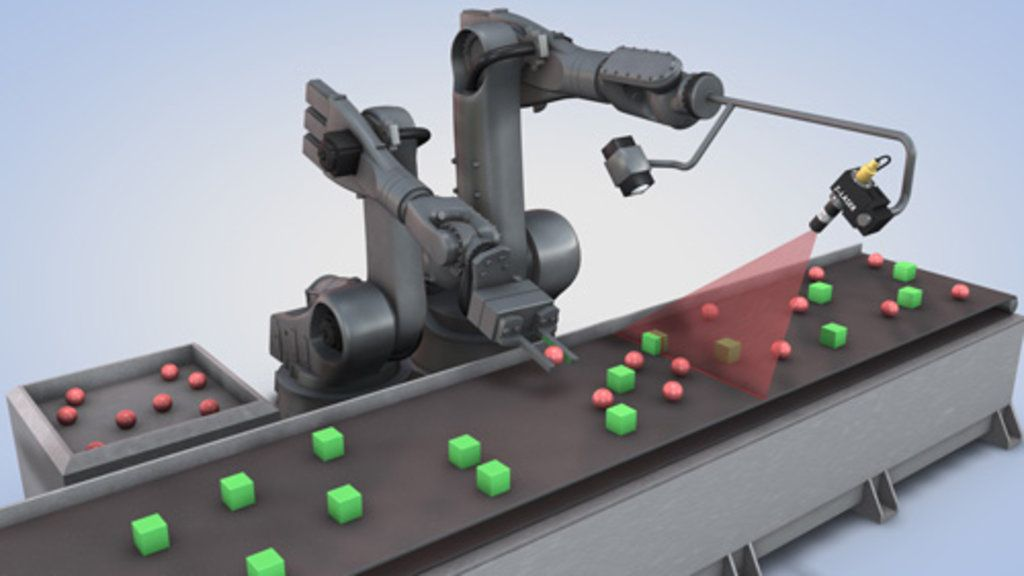
\includegraphics[scale=.55]{./Figures/visionArtificial.jpg}
	\caption{Utilización de visión artificial en la industria\protect\footnotemark.}
	\label{fig:visionArtificial}
\end{figure}

\footnotetext{Imagen tomada de \url{https://www.z-laser.es/aplicaciones/robotica.html}}

\newpage

Los sistemas de visión artificial se utilizan actualmente en diferentes ámbitos o industrias, como por ejemplo:
\begin{itemize}
\item En metrología: lo que hasta ahora se venía realizando con complejos equipos de metrología láser, se puede medir utilizando la visión artificial.
\item Detección de intrusos: se utiliza visión artificial para separar objetos no deseados en una línea transportadora, por ejemplo, remover ramas de una línea transportadora de frutas.
\item Verificación de montaje: se utiliza visión artificial para verificar el correcto montaje de un equipo o garantizar que no haya faltantes en una línea de montaje.
\item Sector médico: se utiliza visión artificial para apoyar al profesional médico y simplificar procesos de análisis de células cancerígenas, lunares y radiografías.
\item Sector automotriz: se utiliza visión artificial como un sistema que monitorea el tránsito y las condiciones de manejo, con el objetivo de evitar o reducir accidentes actuando en conjunto con otros sistemas de seguridad.
\end{itemize}

\subsection{Visión por computadora}

La visión artificial o visión por computadora \textit{(computer vision)} \citep{COMPUTER_VISION} es una rama de la ciencia de la computación que desarrolla métodos para adquirir, procesar y analizar imágenes del mundo real, con el fin de que una máquina pueda interpretarlas. Esta disciplina implementa herramientas de detección de patrones (líneas, bordes, texturas) llamadas filtros digitales. En la figura \ref{fig:visionComputadora} se observa un ejemplo del uso del ``algoritmo de Canny'' para la detecciones de bordes en una imagen.

\begin{figure}[ht]
	\centering
	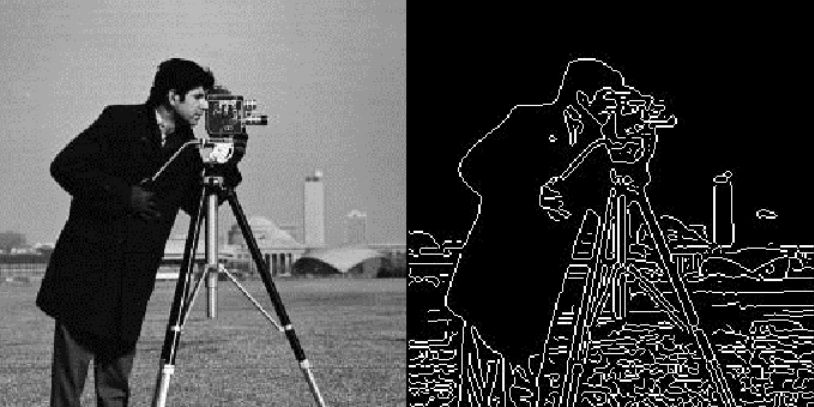
\includegraphics[scale=.55]{./Figures/visionComputadora.jpg}
	\caption{Filtro de Canny de visión por computadora\protect\footnotemark.}
	\label{fig:visionComputadora}
\end{figure}


\footnotetext{Imagen tomada de \url{https://www.researchgate.net/figure/The-Canny-Edger-on-the-image-Cameraman_fig13_266832526}}

Hasta principios de la década del 2010, los filtros clásicos de visión por computadora eran las herramientas más populares para analizar imágenes en la industria. En el 2012, con los primeros modelos de aprendizaje profundo para visión, la forma en la cual se trabaja y analiza las imágenes cambió drásticamente, abriendo un nuevo mundo de técnicas y posibilidades a la industria.

\newpage

\subsection{Aprendizaje profundo}

El aprendizaje profundo o \textit{Deep Learning} \citep{DEEP_LEARNING} es un subcampo de la inteligencia artificial, el cual utiliza distintas estructuras de redes neuronales para lograr representaciones de los datos cada vez más significativas. Las redes neuronales son un modelo computacional basado en un gran conjunto de unidades neuronales simples (neuronas artificiales), inspirado en el comportamiento observado de las neuronas en los cerebros humanos. 

Las técnicas de aprendizaje profundo combinadas con las técnicas de visión por computadora crearon las redes convolucionales. La arquitectura actual de redes convolucionales creada en 2012 revolucionó el campo del análisis de imágenes y video. En la figura \ref{fig:visionDeepLearning} se observan algunas de las técnicas de visión por aprendizaje profundo más populares, entre las que se encuentran: clasificación, detección y segmentación de imágenes.

\begin{figure}[ht]
	\centering
	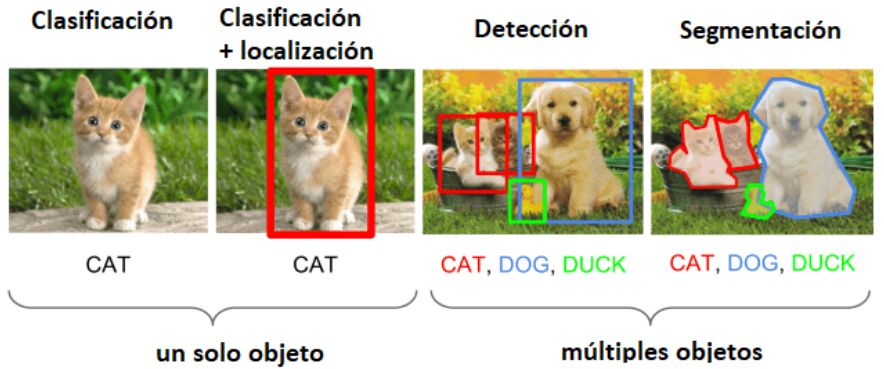
\includegraphics[scale=.7]{./Figures/visionDeepLearning.jpg}
	\caption{Técnicas de redes convolucionales en aprendizaje profundo\protect\footnotemark.}
	\label{fig:visionDeepLearning}
\end{figure}

\footnotetext{Imagen tomada de \url{https://ml4a.github.io/ml4a/convnets/}}

%----------------------------------------------------------------------------------------
%	SECTION 2
%----------------------------------------------------------------------------------------

\section{Motivación}
\label{sec:motivacion}

Una de las principales motivaciones en la realización de este trabajo es la adopción de las nuevas tecnologías de aprendizaje profundo en la industria y el  creciente desarrollo de estas. La incorporación de estas nuevas tecnologías permiten crear soluciones para monitorear condiciones en ambientes más adversos, como es el monitoreo de personas en una tienda.

Globant S.A. busca utilizar estas tecnologías para transformar las organizaciones, cambiando la forma en que estas se conectan con los usuarios buscando potenciar sus experiencias de consumo.

\newpage

%----------------------------------------------------------------------------------------
%	SECTION 3
%----------------------------------------------------------------------------------------

\section{Estado del arte}
\label{sec:estadoDelArte}

A partir de la la década del 2010, la mayor cantidad de documentos científicos en el ámbito de la ciencia de la computación están enfocados en inteligencia artificial, que supera por mucho la cantidad de publicaciones de las otras ramas de esta ciencia \citep{AI_PAPERS}. El creciente desarrollo de la inteligencia artificial y su incorporación en la industria es posible gracias al avance del hardware, que hace posible ejecutar software más complejo, en tiempo real, pudiendo crear nuevas soluciones.

En la figura \ref{fig:cpuGPU} se observa como han evolucionado las unidades de procesamiento gráfico (GPU) que hicieron posible esta nueva ola de desarrollo en el campo de la inteligencia artificial.

\begin{figure}[ht]
	\centering
	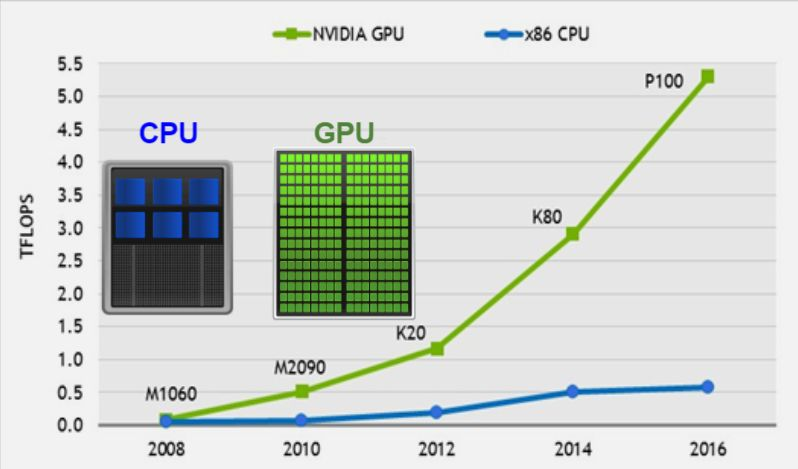
\includegraphics[scale=.8]{./Figures/cpuGPU.jpg}
	\caption{Evolución de las GPUs y CPUs\protect\footnotemark.}
	\label{fig:cpuGPU}
\end{figure}

\footnotetext{Imagen tomada de \url{https://www.networld.co.jp/files/9615/0846/8069/GPUs_Data_Analytics_Book.pdf}}

En la figura \ref{fig:cpuGPU} se compara la cantidad de operaciones de punto flotante por segundo (TFLOPS) \citep{TFLOPS} que pueden efectuar las GPUs y CPUs más modernas. Actualmente, una GPU puede contener 200 veces más núcleos que una CPU, permitiendo lograr más operaciones matemáticas simples por segundo. Los algoritmos de aprendizaje profundo se desarrollaron teniendo en consideración las operaciones que pueden ejecutar y paralizar las GPUs, lo que posibilita su ejecución en tiempo real.

El creciente desarrollo de la inteligencia artificial viene acompañado por el fenómeno de ``big data''. Actualmente, la cantidad de información que se produce supera la cantidad de información generada en toda la historia de la humanidad. Esto es posible ya que todas las personas están interactuando constantemente con la nube mediante dispositivos conectados a internet (redes sociales, foros, juegos). A todo este ecosistema se suma internet de las cosas (IoT), en donde los dispositivos (sensores, computadoras, cámaras) recolectan y suben información constantemente a la nube para el monitoreo y control de sistemas, casas y productos.

\newpage

Acompañando el crecimiento tecnológico surgieron en el mercado nuevas soluciones de monitoreo de personas, basadas en técnicas de visión por aprendizaje profundo (detección y seguimiento de objetos en imágenes) . Estas técnicas no requieren utilizar cámaras de alta resolución y pueden llegar a ejecutarse dentro de un dispositivo embebido o un celular.

Entre las soluciones disponibles en el mercado se pueden encontrar los siguientes servicios:
\begin{itemize}
\item Contar la cantidad de personas que entran y salen del recinto.
\item Indicar en tiempo real el nivel de ocupación.
\item Administrar múltiples filas de espera, ayudando al personal a distribuir de forma eficiente a los clientes.
\item Recomendaciones respecto a las áreas más transitadas del recinto, con el objetivo de ayudar al personal a optimizar el flujo de tránsito.
\end{itemize}

Los beneficios que se obtienen de la utilización de estos sistemas en tiendas o supermercados también pueden extenderse a eventos, bancos, hoteles, edificios inteligentes o cualquier industria en donde la logística y el manejo del espacio sean vitales para su negocio.

%----------------------------------------------------------------------------------------
%	SECTION 4
%----------------------------------------------------------------------------------------

\section{Objetivos y alcance}
\label{sec:objetivosAlcance}

\subsection{Objetivos}

El propósito de este trabajo fue el desarrollo de un sistema de monitoreo de personas. Tiene como principal objetivo estudiar los movimientos que realiza un individuo al ingresar y transitar un espacio a fin de obtener métricas sobre las zonas que visitó. Para poder cumplir este objetivo es necesario poder detectar a las personas que aparecen en el video tomado por una cámara, realizar el seguimiento de cada una y poder identificarlas aún cuando desaparecen del espacio de visión por unos segundos.

En la figura \ref{fig:esquemaGeneral} se observa un diagrama general de la solución y las etapas que la componen.

\begin{figure}[ht]
	\centering
	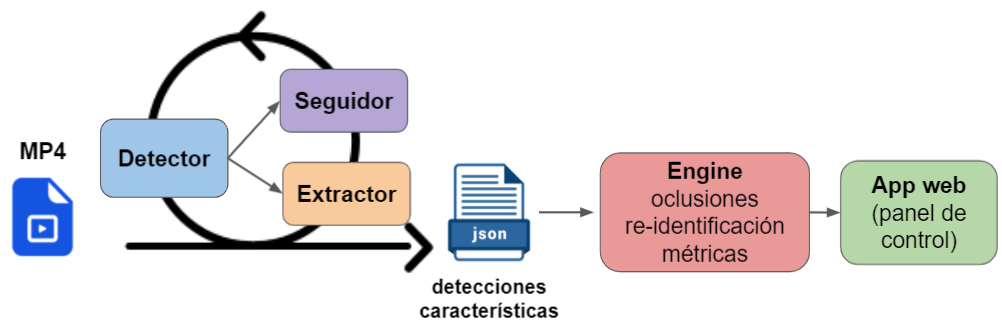
\includegraphics[scale=.6]{./Figures/esquemaGeneral.png}
	\caption{Diagrama general de la solución.}
	\label{fig:esquemaGeneral}
\end{figure}

El detector, seguidor y extractor son modelos de inteligencia artificial que utilizan técnicas de aprendizaje profundo, encargados de detectar y seguir a las personas en un video. El resultado de esta etapa es un archivo con las detecciones y características de cada persona monitoreada. 

El ``Engine'' es la parte del sistema encargada de mejorar la precisión de seguimiento mediante re-identificación y manejo de oclusiones. Además, calcula las métricas de monitoreo que luego se presentan en la interfaz de usuario disponible en la aplicación web.

En el capítulo \ref{Chapter3} se detalla el diseño y la implementación de las etapas que componen a este sistema.

\subsection{Alcance}

Para la elaboración de este trabajo, la parte del sistema involucrada con aprendizaje profundo se ejecutó en una plataforma que proporciona una GPU para la ejecución de los modelos. La otra parte del sistema, el ``Engine'' y la aplicación web, se ejecutaron en una máquina personal. El desarrollo de las etapas mencionadas incluye los siguientes aspectos:
\begin{itemize}
\item Implementación de una cadena de procesamiento de inteligencia artificial que consuma videos \file{.mp4} y detecte personas.
\item Implementación de un sistema de mejora de monitoreo (``Engine''), que aborde los problemas de oclusiones y re-identificación de personas.
\item Implementación de una aplicación web para la configuración general del sistema.
\item Visualización de los datos en tiempo real en la aplicación web.
\item Alcanzar los requerimientos de monitoreo de personas establecidos en la sección \ref{sec:requerimientos}.
\end{itemize}

La plataforma que se seleccionó para ejecutar los modelos de inteligencia artificial con GPU es \textit{Google Colaboratory (Colab)}, la cual permite a cualquier usuario utilizar los recursos de Google de forma gratuita durante un tiempo limitado. Las limitaciones sobre los recursos de Colab no afectan la elaboración de este trabajo, ya que no es parte del alcance la implementación en tiempo real de los modelos de inteligencia artificial.


